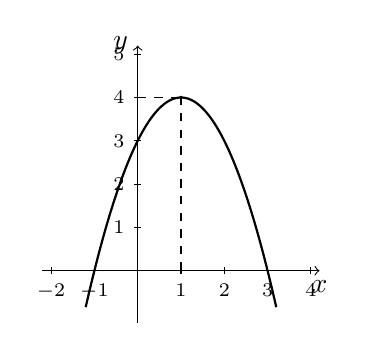
\begin{tikzpicture}[scale=0.55]
    \draw[->] (-2.2,0) -- (4.2,0) node[below] {$x$};
    \draw[->] (0,-1.2) -- (0,5.2) node[left] {$y$};
    \foreach \x in {-2,-1,1,2,3,4}
        \draw (\x,0.08) -- (\x,-0.08) node[below] {\scriptsize $\x$};
    \foreach \y in {1,2,3,4,5}
        \draw (0.08,\y) -- (-0.08,\y) node[left] {\scriptsize $\y$};
    \draw[smooth, samples=200, domain=-1.2:3.2, thick] plot (\x, {-(\x-1)^2+4});
    \fill (1,4) circle (1.2pt);
    \draw[dashed] (1,0) -- (1,4);
    \draw[dashed] (0,4) -- (1,4);
\end{tikzpicture}
